\documentclass{beamer}
\usetheme{CambridgeUS}
\usepackage[utf8]{inputenc}
\usepackage{tikz}
\usetikzlibrary{quotes} % LATEX and plain TEX
\usetikzlibrary{arrows,automata,positioning}

\usetikzlibrary{shapes.geometric}



\title{1-2-3 Domneva}

\author{Gašper Domen Romih}

\date{\today}

\begin{document}
\begin{frame}
	\titlepage
\end{frame}
\begin{frame}
\tableofcontents
\end{frame}
\section{Osnovne definicije}

\begin{frame}
\begin{block}{Graf}
Graf $G$ je urejen par $(V, E)$, kjer je množica $V$ množice vozlišč in $E \subset V^2$ množice povezav.
\end{block}

\begin{block}{Barvanje grafa}
	Barvanje grafa $G = (V, E)$ je preslikava $c : V \rightarrow S$. Množici $S$ rečemo množica barv. Rečemo, da je barvanje \textbf{pravilno}, če za vsak $uv \in E$ velja $c(u) \neq c(v)$.
\end{block}
\begin{block}{Utežitev grafa}
	Utežitev grafa je preslikava $\omega : E \rightarrow W$. V kolikor je množica uteži $W$ oblike $\{1,2,\ldots, k\}$ rečemo, da je preslikava $\omega$ $k$-utežitev grafa $G$.
\end{block}
\end{frame}

\begin{frame}{Od utežitve do barvanja}
\begin{block}{Barvanje grafa z $k$-utežitvijo}
	Naj bo $\omega$ neka $k$-utežitev grafa $G$. Sedaj definiramo preslikavo $c_{\omega} : V \rightarrow S$ na naslednji način:
	$$ c_{\omega}(u) = \sum_{e = uv \in E} \omega(e). $$
\end{block}
\begin{figure}
			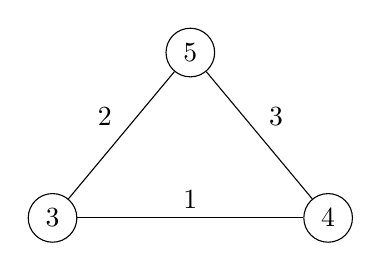
\begin{tikzpicture}
	[scale=.7,auto=left,main node/.style={shape=circle,draw,fill=white}]
	\node [main node] (1) at (0,0) {3};
	\node [main node] (2) at (5,0) {4};
	\node [main node] (3) at (2.5,3) {5};
	
	
	\path[]
	(1) edge node {1} (2)
	(1) edge node {2} (3)
	(2) edge node [above right] {3} (3)
	
	;
	
	
	
	\end{tikzpicture}
	\caption{Primer $3$-utežitve, ki porodi pravilno $3$-barvanje.}
\end{figure}

\end{frame}

\section{1-2-3 Domneva}
\begin{frame}
\begin{block}{}
	Označimo z $\mu(G)$ najmanjši tak $k$ za katerega obstaja $k$-utežitev $\omega$ grafa $G$, ki inducira pravilno barvanje $c_{\omega}$.
\end{block}
\begin{block}{1-2-3 Domneva}
	Za vsak povezan graf $G$, ki ni $K_2$ je $\mu(G) \le 3$.
\end{block}
\end{frame}

\subsection{Zgodovinski okvir}
\begin{frame}
\begin{itemize}
	\item Leta 2004 v članku [] zastavljena domneva.
	\item Leta 2007 dokazano $\mu(G) \le 30$.
	\item Leta 2008 dokazano $\mu(G) \le 16$.
	\item Leta 2008 dokazano $\mu(G) \le 13$.
	\item Leta 2009 $\mu(G) \le 6$.
	\item Leta 2010 $\mu(G) \le 5$. To je do sedaj tudi najboljši rezultat za splošne grafe.
\end{itemize}

\begin{block}{Opomba}
	Kljub temu, da je trenutno najboljša zgornja $\mu(G) \le 5$ je za veliko zananih družin grafov dokazano $\mu(G) \le 3$. 
\end{block}
\end{frame}

\subsection{Izračun $\mu$ za poti}
\begin{frame}{$\mu(P_n)$ za $n \le 3$}
V primeru $n=2$ imamo graf $K_n$ zato obravnavamo primere ko $n \ge 3$.  Posebaj si oglejmo še primer ko $n = 3$.  V tem primeru utežimo povezavi z $1$ in dobimo pravilno barvanje iz česar sledi $\mu(P_3) = 1$.

\begin{figure}[!h]
	\centering
	\label{fig:pn}
	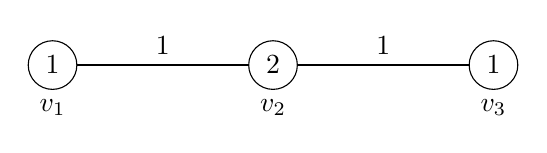
\begin{tikzpicture}
	[scale=.7,auto=left,main node/.style={shape=circle,draw,fill=white}]
	\node [main node] (1) at (1,1) [label=below:$v_1$] {1} ;
	\node [main node](2) at (5,1) [label=below:$v_2$] {2} ;
	\node [main node](3) at (9,1) [label=below:$v_3$] {1} ;
	
	
	\path[draw,thick]
	(1) edge node {1} (2)
	(2) edge  node {1} (3)
	
	;
	
	\end{tikzpicture}
	\caption{Primer utežitve grafa $P_n$.}
\end{figure}
\end{frame}

\begin{frame}{$\mu(P_n)$ za $n > 3$}
	Najprej oštevilčimo povezave kot $e_1, e_2, \ldots, e_{n-1}$, kjer $e_i = v_i v_{i+1}$ za $1 \le i < n$.
	\begin{block}{Pogoj za pravilno barvanje}
		Utežitev povezav $\omega$ inducira pravilno barvanje $P_n$ natanko tedaj ko $\omega(e_i) \neq \omega(e_j)$ za vsak $|j -i| = 2$.
	\end{block}
\begin{figure}[!h]
	\centering
	\label{fig:pn}
	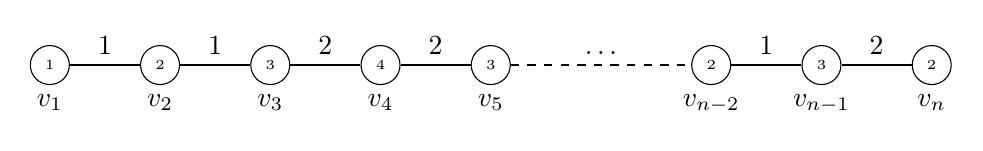
\begin{tikzpicture}
	[scale=.7,auto=left,main node/.style={shape=circle,draw,fill=white}]
	\node [main node] (1) at (1,1) [label=below:$v_1$] {\tiny 1} ;
	\node [main node](2) at (3,1) [label=below:$v_2$] {\tiny 2} ;
	\node [main node](3) at (5,1) [label=below:$v_3$] {\tiny 3} ;
	\node [main node](4) at (7,1) [label=below:$v_4$] {\tiny 4} ;
	\node [main node](5) at (9,1) [label=below:$v_5$] {\tiny 3} ;
	
	\node [main node](6) at (13,1) [label=below:$v_{n-2}$] {\tiny 2} ;
	\node [main node](7) at (15,1) [label=below:$v_{n-1}$] {\tiny 3} ;
	\node [main node](8) at (17,1) [label=below:$v_n$]  {\tiny 2};
	
	
	\path[draw,thick]
	(1) edge node {1} (2)
	(2) edge  node {1} (3)
	(3) edge  node {2} (4)
	(4) edge  node {2} (5)
	
	(5) edge [dashed]  node {$\ldots$} (6)
	
	(6) edge  node {1} (7)
	(7) edge  node {2} (8)
	;
	
	\end{tikzpicture}

\end{figure}
\end{frame}

\begin{frame}{Ugotovitve za $P_n$}
	\begin{block}{Utežitev $\omega$ za $P_n$}
		$$
		\omega(e_i) = \begin{cases}
			1 &i \equiv 1,2 \pmod{4}\\ 
			2 &i \equiv 3,4 \pmod{4}
		\end{cases}
		$$
	\end{block}
	\begin{itemize}
		\item Našli smo $2$-utežitev, ki porodi pravilno barvanje $\implies$  $\mu(P_n) = 2$.
		\item Zaporedje uteži na povezavah je $11221\ldots 22112$, lahko pa bi definicijo utežitve popravili z naprimer levim zamikom zgornjega zaporedja. To so tudi vse možne pravilne $2$-utežitve poti.
	\end{itemize}
\end{frame}

\subsection{Izračun $\mu$ za cikle}
\begin{frame}{Osnovna ideja za izračun $\mu(C_n)$}
	\begin{block}{Ideja}
		Cikel je pot, ki ji dodamo povezavo $e_n$ med prvim in zadnjih vozliščem. Pogoj za pravilno barvanje poti velja tudi za cikle . Poizkusili bomo modificirati obstoječo utežitev za poti, tako da boveljavna tudi za cikle.
	\end{block}

\begin{figure}
	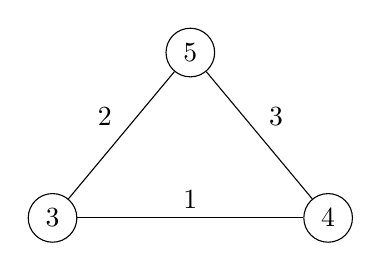
\begin{tikzpicture}
	[scale=.7,auto=left,main node/.style={shape=circle,draw,fill=white}]
	\node [main node] (1) at (0,0) {3};
	\node [main node] (2) at (5,0) {4};
	\node [main node] (3) at (2.5,3) {5};
	
	
	\path[]
	(1) edge node {1} (2)
	(1) edge node {2} (3)
	(2) edge node [above right] {3} (3)
	
	;
	
	
	
	\end{tikzpicture}
	\caption{Na primeru $C_3$ vidimo, $\mu(C_3) = 3$, saj morajo v luči potrebnega pogaja uteži na povezavah biti paroma različne.}
\end{figure}
\end{frame}

\begin{frame}{$\mu(C_n)$ za $n = 4k$}
	Vzamemo kar enako utežitev kot za pot, z dodatkom $\omega(e_n) = 2$.
	\begin{figure}
		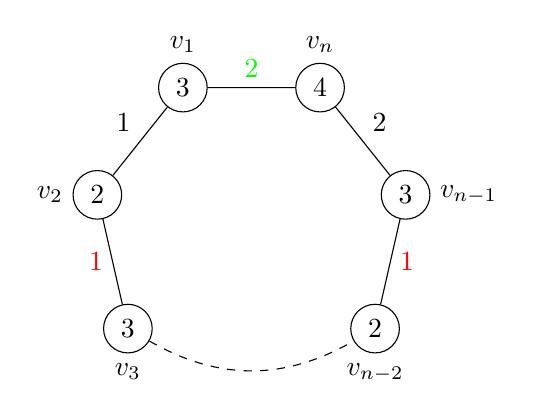
\begin{tikzpicture}
		
		[scale=.8,auto=left,main node/.style={draw=none,fill=none}]
		\def \n {7}
		\node[
		regular polygon,
		regular polygon sides=\n,
		minimum size=4cm,
		rotate=180/\n,
		] (a) {};
		
		\node[draw,shape=circle,fill=none] (1) at (a.corner 1) [label=above:$v_1$] { $3$};
		\node[draw,shape=circle,fill=none] (2) at (a.corner 2) [label=left:$v_2$] { $2$};
		\node[draw,shape=circle,fill=none] (3) at (a.corner 3) [label=below:$v_3$]{ $3$};
		
		\node[draw,shape=circle,fill=none] (4) at (a.corner 5) [label=below:$v_{n-2}$] { $2$};
		\node[draw,shape=circle,fill=none] (5) at (a.corner 6) [label=right:$v_{n-1}$] { $3$};
		\node[draw,shape=circle,fill=none] (6) at (a.corner 7) [label=above:$v_n$]{ $4$};
		
		\draw[] (1) to node [above left] {1}  (2);
		\draw[] (2) to node [text=red,left] {1}  (3);
		\draw[bend right, dashed] (3) to node [] {}  (4);
		\draw[] (4) to node [text=red, right] {1}  (5);
		\draw[] (5) to node [above right] {2}  (6);
		
		\draw[] (6) to node [text=green,above] {2}  (1);
		\end{tikzpicture}
		\caption{Kot je razvidno iz slike zgornja utežitev porodi pravilno barvanje. Na povezavo $e_n$ (označena rdeče) tako vplivata le povezavi $e_2$ in $e_{n-2}$ (označena zeleno). Iz tega sledi $\mu(c_{4k}) = 2$.}
	\end{figure}
\end{frame}

\begin{frame}{$\mu(C_n)$ za $n = 4k + 1$}
Ponovno vzamemo utežitev za pot ter dodamo $\mu(e_n) = 3$.
	\begin{figure}
	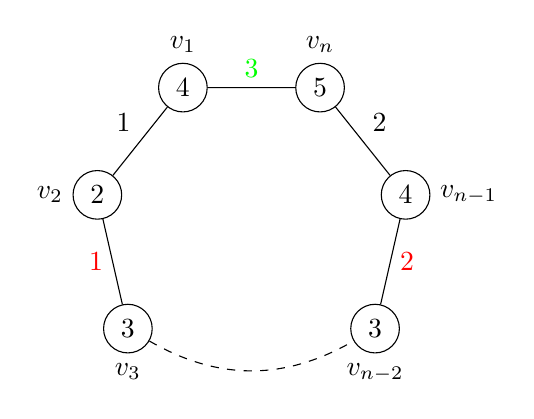
\begin{tikzpicture}
	
	[scale=.8,auto=left,main node/.style={draw=none,fill=none}]
	\def \n {7}
	\node[
	regular polygon,
	regular polygon sides=\n,
	minimum size=4cm,
	rotate=180/\n,
	] (a) {};
	
	\node[draw,shape=circle,fill=none] (1) at (a.corner 1) [label=above:$v_1$] { $4$};
	\node[draw,shape=circle,fill=none] (2) at (a.corner 2) [label=left:$v_2$] { $2$};
	\node[draw,shape=circle,fill=none] (3) at (a.corner 3) [label=below:$v_3$]{ $3$};
	
	\node[draw,shape=circle,fill=none] (4) at (a.corner 5) [label=below:$v_{n-2}$] { $3$};
	\node[draw,shape=circle,fill=none] (5) at (a.corner 6) [label=right:$v_{n-1}$] { $4$};
	\node[draw,shape=circle,fill=none] (6) at (a.corner 7) [label=above:$v_n$]{ $5$};
	
	\draw[] (1) to node [above left] {1}  (2);
	\draw[] (2) to node [text=red,left] {1}  (3);
	\draw[bend right, dashed] (3) to node [] {}  (4);
	\draw[] (4) to node [text=red, right] {2}  (5);
	\draw[] (5) to node [above right] {2}  (6);
	
	\draw[] (6) to node [text=green,above] {3}  (1);
	\end{tikzpicture}
	\caption{Kot je razvidno iz slike zgornja utežitev porodi pravilno barvanje. Nova povezava sedaj zaradi omejitev ne more imeti uteži $1$ ali $2$. Utež 3 na povezavi $e_n$ tako porodi pravilno barvanje iz česar sledi $\mu(C_{4k + 1}) \le 3$.}
\end{figure}
\end{frame}

\begin{frame}{$\mu(C_n)$ za $n=4k + 2$}
	Poleg povezave $e_n$ moramo v tem primeru popravit tudi $e_{n-1}$.
	
		\begin{figure}
		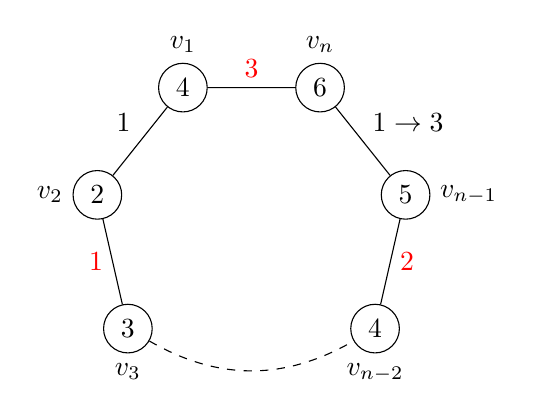
\begin{tikzpicture}
		
		[scale=.8,auto=left,main node/.style={draw=none,fill=none}]
		\def \n {7}
		\node[
		regular polygon,
		regular polygon sides=\n,
		minimum size=4cm,
		rotate=180/\n,
		] (a) {};
		
		\node[draw,shape=circle,fill=none] (1) at (a.corner 1) [label=above:$v_1$] { $4$};
		\node[draw,shape=circle,fill=none] (2) at (a.corner 2) [label=left:$v_2$] { $2$};
		\node[draw,shape=circle,fill=none] (3) at (a.corner 3) [label=below:$v_3$]{ $3$};
		
		\node[draw,shape=circle,fill=none] (4) at (a.corner 5) [label=below:$v_{n-2}$] { $4$};
		\node[draw,shape=circle,fill=none] (5) at (a.corner 6) [label=right:$v_{n-1}$] { $5$};
		\node[draw,shape=circle,fill=none] (6) at (a.corner 7) [label=above:$v_n$]{ $6$};
		
		\draw[] (1) to node [above left] {1}  (2);
		\draw[] (2) to node [text=red,left] {1}  (3);
		\draw[bend right, dashed] (3) to node [] {}  (4);
		\draw[] (4) to node [text=red, right] {2}  (5);
		\draw[] (5) to node [above right] {$1 \to 3$}  (6);
		
		\draw[] (6) to node [text=red,above] {3}  (1);
		\end{tikzpicture}
		\caption{Kot v prjšnjem primer moramo nastavit utež na povezavi $e_n$ na 3. Ker ima povezava $e_1$ enako utež kot $e_{n-1}$ popravimo še utež na tej povezavi na 3. }
	\end{figure}
\end{frame}

\begin{frame}{$\mu(C_n)$ za $n = 4k + 3$}
	V tem primeru moramo prav tako popravit uteži na dveh povezavah. Deluje kar isti popravek kot v prejšnjem primeru.
	
		\begin{figure}
		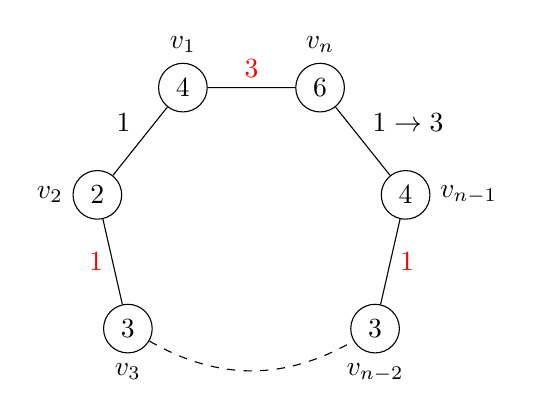
\begin{tikzpicture}
		
		[scale=.8,auto=left,main node/.style={draw=none,fill=none}]
		\def \n {7}
		\node[
		regular polygon,
		regular polygon sides=\n,
		minimum size=4cm,
		rotate=180/\n,
		] (a) {};
		
		\node[draw,shape=circle,fill=none] (1) at (a.corner 1) [label=above:$v_1$] { $4$};
		\node[draw,shape=circle,fill=none] (2) at (a.corner 2) [label=left:$v_2$] { $2$};
		\node[draw,shape=circle,fill=none] (3) at (a.corner 3) [label=below:$v_3$]{ $3$};
		
		\node[draw,shape=circle,fill=none] (4) at (a.corner 5) [label=below:$v_{n-2}$] { $3$};
		\node[draw,shape=circle,fill=none] (5) at (a.corner 6) [label=right:$v_{n-1}$] { $4$};
		\node[draw,shape=circle,fill=none] (6) at (a.corner 7) [label=above:$v_n$]{ $6$};
		
		\draw[] (1) to node [above left] {1}  (2);
		\draw[] (2) to node [text=red,left] {1}  (3);
		\draw[bend right, dashed] (3) to node [] {}  (4);
		\draw[] (4) to node [text=red, right] {1}  (5);
		\draw[] (5) to node [above right] {$1 \to 3$}  (6);
		
		\draw[] (6) to node [text=red,above] {3}  (1);
		\end{tikzpicture}
		\caption{Na enak način kot v prejšnjem primeru dobimo pravilno barvanje. }
	\end{figure}
\end{frame}

\begin{frame}{Ugotovitve za $C_n$}
	Ugotovili smo, da $\mu(C_n) \le 3$ za vsak $n$. Pokazali bomo še, da je ta meja tudi stroga za $n \neq 4k$. Recimo nasprotno torej, da imamo $2$-utežitev cikla, ki porodi pravilno barvanje. Veljati mora torej $\omega(e_i) \neq \omega(e_{i + 2})$ iz česar sledi $\omega(e_i) = \omega(e_{i + 4})$. To pa je protislovje ko $n \neq 4k$.
	\begin{block}{Rezultat}
		
		Za $C_n$ velja:
		$$ 
		\mu(C_n) = 
		\begin{cases}
		2; \text{ } n \equiv 0 \pmod{4} \\
		3; \text{ sicer}
		\end{cases}
		$$
	\end{block}
\end{frame}


\end{document}